\pdfminorversion=7
\documentclass{article}
\usepackage[paperwidth=183mm,paperheight=252mm,margin=2.5mm]{geometry}
\usepackage{graphicx}
\usepackage{tikz}
\pagestyle{empty}
\setlength{\parindent}{0pt}

\begin{document}
\begin{tikzpicture}[remember picture, overlay,
                    every node/.style={anchor=north west, inner sep=0pt}]

  % Row 1: global donor landscape (b)
  \node at (3mm, -4mm) {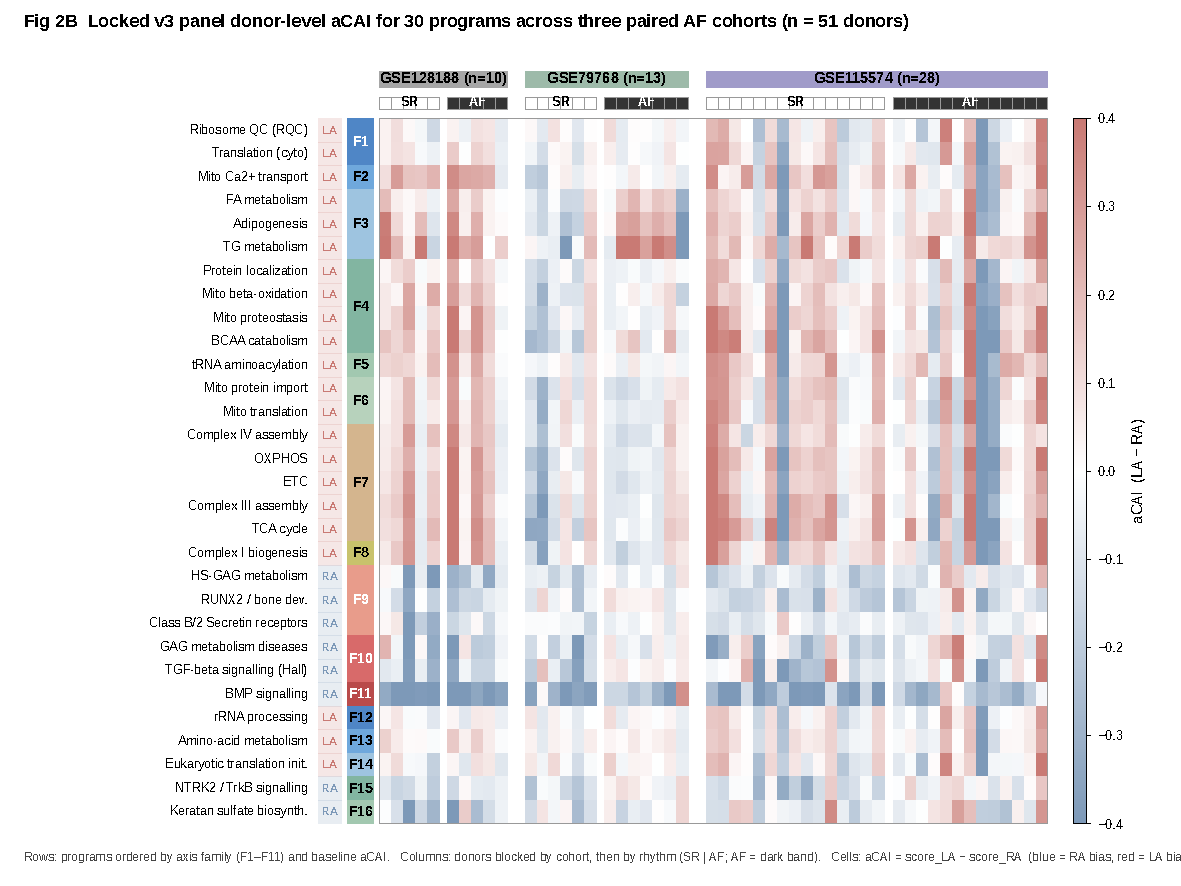
\includegraphics[width=177mm]{fig2b_donor_acai_heatmap_v3.pdf}};

  % Row 2: decomposition + forest + replication (c / d / e)
  \node at (3mm,   -142mm) {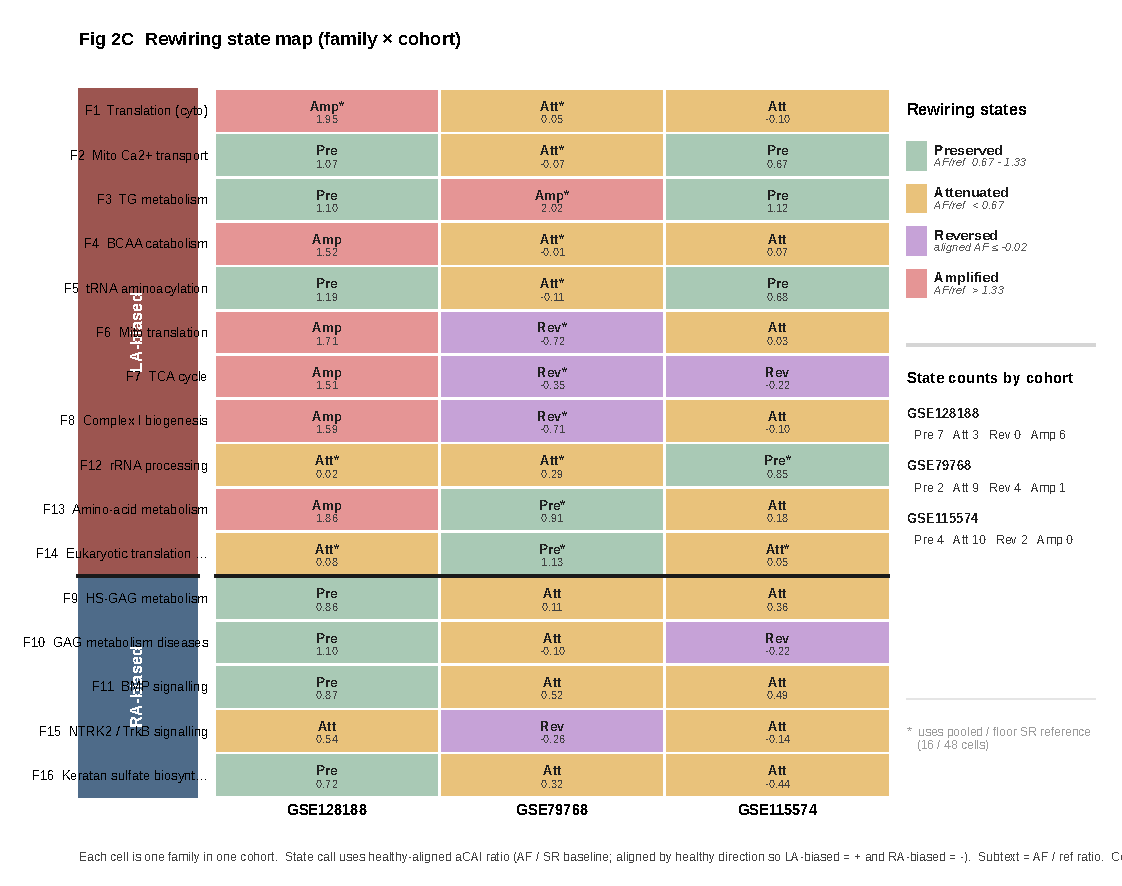
\includegraphics[width=58mm]{fig2c_chamber_decomposition_v3.pdf}};
  \node at (64mm,  -142mm) {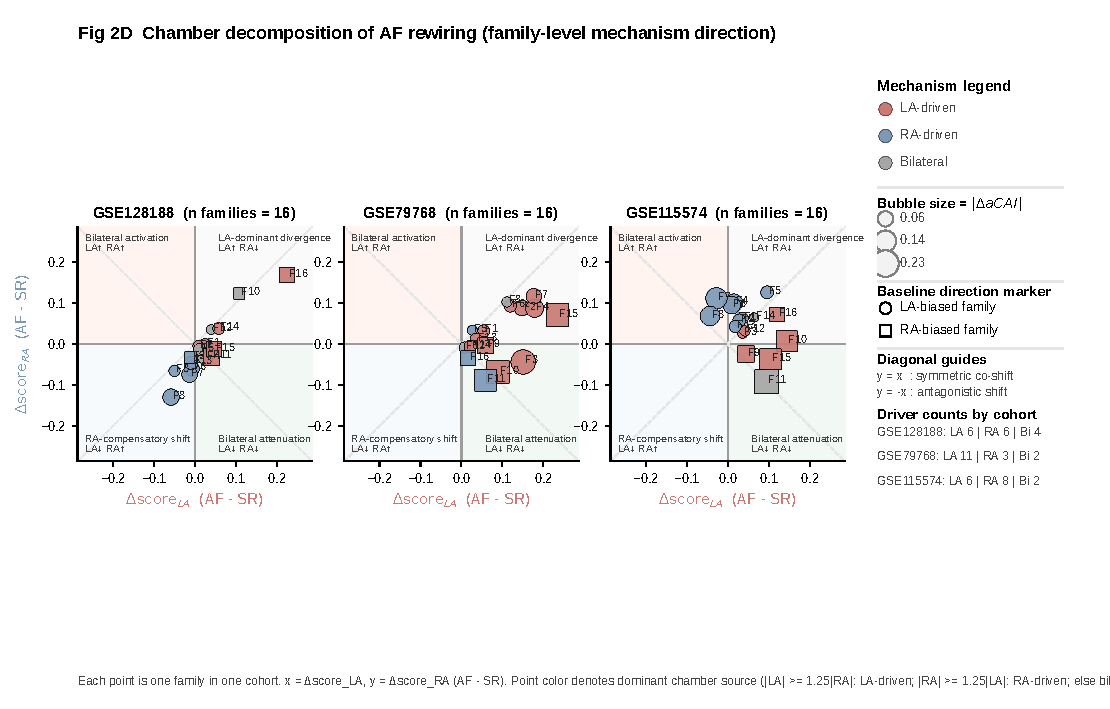
\includegraphics[width=58mm]{fig2d_family_forest_v3.pdf}};
  \node at (125mm, -142mm) {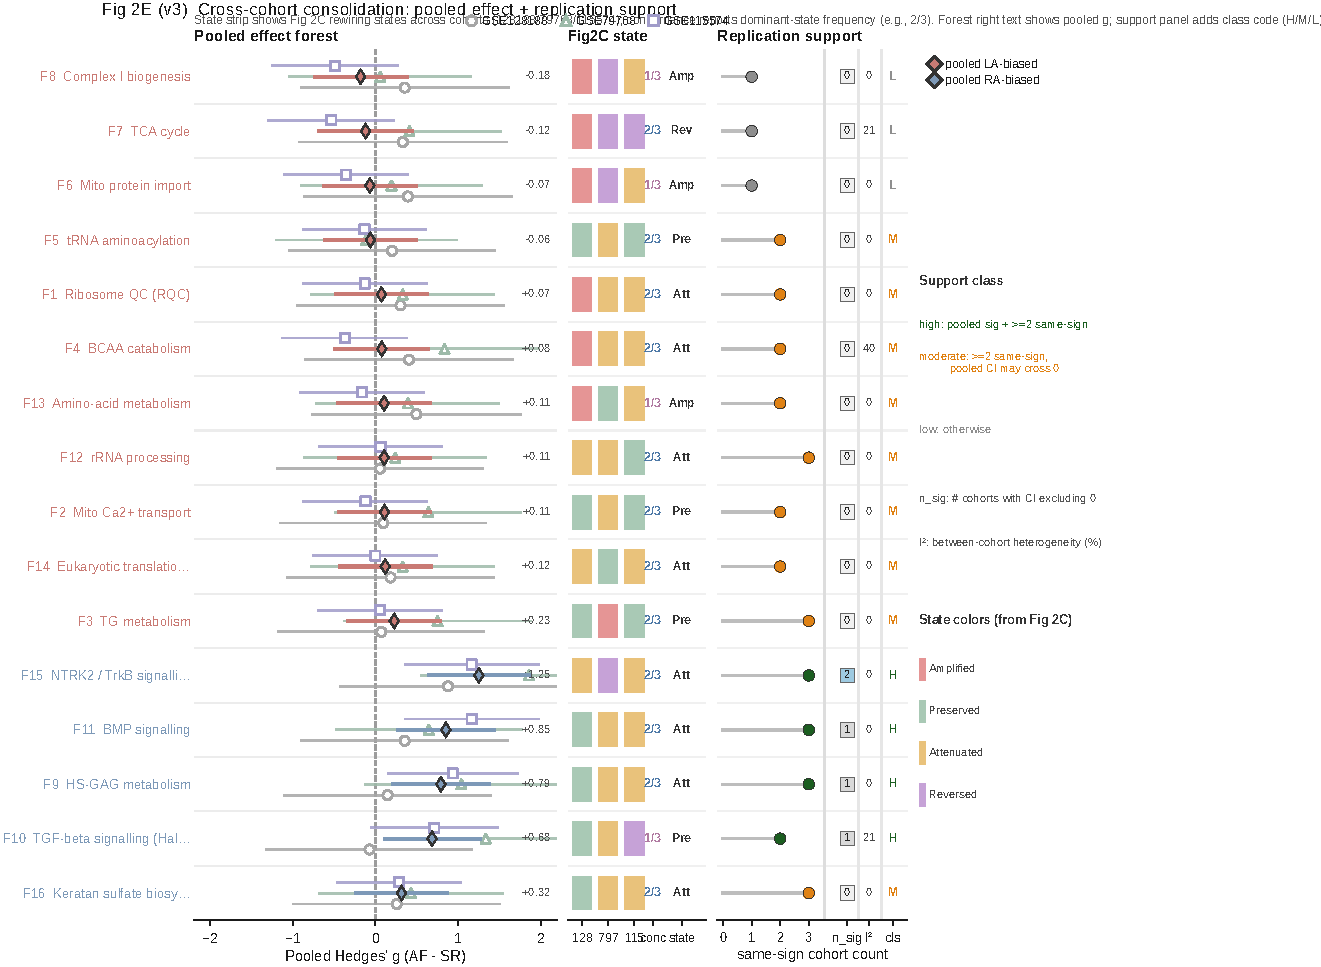
\includegraphics[width=58mm]{fig2e_replication_lollipop_v3.pdf}};

\end{tikzpicture}
\end{document}
